\documentclass[a4paper,12pt]{report}

% --- Encoding & Font ---
\usepackage[utf8]{inputenc}
\usepackage[T5,T1]{fontenc}
\usepackage[vietnamese,english]{babel}
\usepackage{times}

% --- Page Layout ---
\usepackage[top=2.5cm, bottom=2.5cm, left=3cm, right=2.5cm]{geometry}
\usepackage{setspace}
\onehalfspacing

% --- Graphics ---
\usepackage{graphicx}
\usepackage{float}
\usepackage{subcaption}

% --- Tables ---
\usepackage{booktabs}
\usepackage{array}
\usepackage{longtable}
\usepackage{multirow}
\usepackage{tabularx}

% --- Math ---
\usepackage{amsmath}
\usepackage{amssymb}

% --- Code Listings ---
\usepackage{listings}
\usepackage{xcolor}

\definecolor{codebg}{RGB}{248,248,248}
\definecolor{codeframe}{RGB}{200,200,200}
\definecolor{codecomment}{RGB}{106,153,85}
\definecolor{codestring}{RGB}{163,21,21}
\definecolor{codekeyword}{RGB}{0,0,255}
\definecolor{ptitblue}{RGB}{0,51,153}

\lstdefinestyle{pythonstyle}{
  language=Python,
  backgroundcolor=\color{codebg},
  frame=single,
  rulecolor=\color{codeframe},
  basicstyle=\ttfamily\footnotesize,
  keywordstyle=\color{codekeyword}\bfseries,
  commentstyle=\color{codecomment}\itshape,
  stringstyle=\color{codestring},
  showstringspaces=false,
  breaklines=true,
  numbers=left,
  numberstyle=\tiny\color{gray},
  numbersep=8pt,
  tabsize=4,
  captionpos=b,
}
\lstset{style=pythonstyle}

% --- Hyperlinks ---
\usepackage[hidelinks]{hyperref}
\usepackage{url}

% --- Section Formatting (UI/UX optimized hierarchy) ---
\usepackage{titlesec}

\titleformat{\chapter}[display]
  {\normalfont\fontsize{22}{26}\bfseries}
  {Chapter \thechapter}{14pt}{\fontsize{22}{26}\bfseries}
\titlespacing*{\chapter}{0pt}{-10pt}{24pt}

\titleformat{\section}
  {\normalfont\fontsize{16}{20}\bfseries}{\thesection}{1em}{}
\titlespacing*{\section}{0pt}{18pt}{10pt}

\titleformat{\subsection}
  {\normalfont\fontsize{13}{17}\bfseries}{\thesubsection}{1em}{}
\titlespacing*{\subsection}{0pt}{14pt}{8pt}

\titleformat{\subsubsection}
  {\normalfont\fontsize{12}{15}\bfseries\itshape}{\thesubsubsection}{1em}{}
\titlespacing*{\subsubsection}{0pt}{10pt}{6pt}

% --- Caption ---
\usepackage{caption}
\captionsetup{font=small, labelfont=bf, skip=8pt}

% --- Header / Footer ---
\usepackage{fancyhdr}
\pagestyle{fancy}
\fancyhf{}
\fancyfoot[C]{\thepage}
\renewcommand{\headrulewidth}{0pt}

% --- TOC depth ---
\setcounter{tocdepth}{3}
\setcounter{secnumdepth}{3}

% --- Indentation ---
\usepackage{indentfirst}
\setlength{\parindent}{1cm}

% --- TikZ for cover page decorations ---
\usepackage{tikz}
\usetikzlibrary{calc}


\begin{document}

% =============================================================
% TITLE PAGE
% =============================================================
\begin{titlepage}
\thispagestyle{empty}

% --- Decorative double-line border with corner ornaments ---
\begin{tikzpicture}[remember picture, overlay]
  % Outer border
  \draw[line width=1.6pt]
    ([shift={(1.2cm,-1.2cm)}]current page.north west)
    rectangle
    ([shift={(-1.2cm,1.2cm)}]current page.south east);
  % Inner border
  \draw[line width=0.5pt]
    ([shift={(1.45cm,-1.45cm)}]current page.north west)
    rectangle
    ([shift={(-1.45cm,1.45cm)}]current page.south east);
\end{tikzpicture}

\begin{center}

% --- University & Department header ---
\textbf{\fontsize{13}{16}\selectfont POSTS AND TELECOMMUNICATIONS INSTITUTE OF TECHNOLOGY}\\[0.25cm]
\textbf{\fontsize{13}{16}\selectfont FACULTY OF INFORMATION TECHNOLOGY}\\[0.15cm]

% --- Dashed separator ---
{\centering\rule[0.5ex]{10cm}{0.4pt}\par}

\vspace{0.8cm}

% --- PTIT Logo ---

\includegraphics[width=3.5cm]{logo.jpg}

\vspace{0.8cm}

% --- Subject title (blue, large, bold, linked to GitHub) ---
{\fontsize{20}{26}\selectfont\bfseries\color{ptitblue}
\href{https://github.com/mynhleeh/Python-Programming-Project.git}{PROJECT REPORT}\\[0.3cm]
\href{https://github.com/mynhleeh/Python-Programming-Project.git}{PYTHON PROGRAMMING}}\\[0.8cm]

% --- Group info ---
{\large\textbf{Class:} \textbf{D24CQCE05-B -- Group 4}}\\[0.6cm]

% --- Member table ---
{\fontsize{11}{14}\selectfont
\textit{Team Members}\\[0.3cm]

\begin{tabular}{l c c}
\textbf{Full Name} & \textbf{Student ID} & \textbf{Assignment} \\[0.15cm]
\hline\\[-0.2cm]
\foreignlanguage{vietnamese}{Lê Anh Minh} & B24DCCE180 & 3 \\[0.1cm]
\foreignlanguage{vietnamese}{Ứng Trọng Trình} & B24DCCE271 & 2 \\[0.1cm]
\foreignlanguage{vietnamese}{Nguyễn Đinh Anh Quân} & B24DCCE222 & 1 \\[0.3cm]
\end{tabular}
}

\vspace{0.8cm}

% --- Instructor ---
{\large\textbf{Instructor:} \foreignlanguage{vietnamese}{MSc. Lê Văn Vịnh}}

\vfill

% --- Footer: City & Year ---
{\large Hanoi, 2026}

\end{center}
\end{titlepage}

% =============================================================
% ABSTRACT
% =============================================================
\chapter*{Abstract}
\addcontentsline{toc}{chapter}{Abstract}

This report presents the complete design and implementation of a data analytics system for football players in the English Premier League, season 2024 -- 2025. The system is structured into three main phases:

\begin{enumerate}
    \item \textbf{Data Crawling:} Match statistics are automatically collected from FBref using SeleniumBase in Undetected Chrome mode, combined with transfer valuations from FootballTransfers via fuzzy string matching. All data is stored in an SQLite database.
    
    \item \textbf{Lookup Application (RESTful API):} A Flask server provides a RESTful API for querying player statistics by name or club, while a command-line client uses the Requests library to retrieve and export results as formatted tables and CSV files.
    
    \item \textbf{Analytics and Machine Learning:} This phase includes descriptive statistics per squad, player clustering using K-Means with PCA visualization, and a player valuation model built with XGBoost and Optuna hyperparameter optimization.
\end{enumerate}

The results demonstrate that the system operates reliably across all three phases, delivering a complete sports analytics pipeline from data acquisition to model evaluation.

% =============================================================
% TABLE OF CONTENTS
% =============================================================
\newpage
\tableofcontents

\newpage
\listoffigures
\addcontentsline{toc}{chapter}{List of Figures}

\newpage
\listoftables
\addcontentsline{toc}{chapter}{List of Tables}


% =============================================================
% CHAPTER 1: INTRODUCTION
% =============================================================
\chapter{Introduction}

\section{Background}

Sports analytics has become an essential field in modern professional football. Top European clubs increasingly rely on quantitative models to evaluate player performance, predict potential, and estimate transfer values. The English Premier League---the highest-revenue club competition in the world---provides a rich and publicly accessible data source well-suited for building analytical systems.

\section{Project Objectives}

This project targets three primary objectives:
\begin{itemize}
    \item Build an automated web scraping system that collects data from multiple online sources, addressing technical challenges such as anti-bot mechanisms and dynamically rendered content.
    \item Design a data query interface in the form of a RESTful API and a command-line application (CLI) supporting flexible lookups.
    \item Apply machine learning techniques including clustering (K-Means) and regression (XGBoost) to discover data structure and predict transfer values.
\end{itemize}

\section{Scope}

Data is limited to players with more than 90 total minutes played in the Premier League 2024--2025 season. Statistical data is sourced from FBref (\url{https://fbref.com}) and transfer valuations from FootballTransfers (\url{https://www.footballtransfers.com}).

\section{Technology Stack}

\begin{table}[H]
\centering
\caption{Summary of technologies and libraries used}
\label{tab:tech_stack}
\begin{tabularx}{\textwidth}{l l X}
\toprule
\textbf{Phase} & \textbf{Library} & \textbf{Brief Role} \\
\midrule
Data Crawling  & SeleniumBase & Anti-bot web crawling \\
               & Pandas       & Data manipulation \\
               & thefuzz      & Fuzzy string matching \\
\midrule
API \& Lookup  & Flask        & API development \\
               & Requests     & HTTP requests \\
               & Tabulate     & Table formatting \\
\midrule
Analytics \& ML & scikit-learn & Clustering \& Scaling \\
               & XGBoost      & Value prediction \\
               & Optuna       & Parameter tuning \\
               & Matplotlib   & Data visualization \\
               & Seaborn      & Statistical charts \\
\midrule
Storage        & SQLite       & Data storage \\
\bottomrule
\end{tabularx}
\end{table}

The detailed description of each library---including its architecture, usage context, and comparison with alternative tools---is provided in the corresponding chapter where it is employed.

\section{Project Structure}

\begin{table}[H]
\centering
\caption{Project directory layout}
\label{tab:project_structure}
\begin{tabularx}{\textwidth}{l X}
\toprule
\textbf{Path} & \textbf{Description} \\
\midrule
\texttt{source\_code/part1/} & Data crawling module \\
\texttt{source\_code/part2/} & API and lookup module \\
\texttt{source\_code/part3/} & Analytics and machine learning module \\
\texttt{source\_code/part3/core/} & Core package: config, loader, features, training, charts \\
\texttt{data/} & Database, CSV outputs, charts \\
\texttt{docs/} & Report and project documentation \\
\bottomrule
\end{tabularx}
\end{table}


% =============================================================
% CHAPTER 2: DATA CRAWLING
% =============================================================
\chapter{Data Crawling}

\section{Objective}

This phase collects two datasets:
\begin{enumerate}
    \item \textbf{Match statistics} for all Premier League 2024--2025 players with more than 90 minutes played, from FBref.
    \item \textbf{Transfer valuations} for each corresponding player from FootballTransfers.
\end{enumerate}

Both datasets are stored in separate tables (\texttt{statistic} and \texttt{price}) within a single SQLite database.

\section{Tools and Libraries}

This section describes the key tools and libraries employed in the data crawling phase, along with the rationale behind each selection.

\subsection{SeleniumBase}

SeleniumBase is a browser automation framework built on top of Selenium WebDriver, designed for web testing and data extraction. Its most distinctive feature is the \textit{Undetected Chrome} (UC) mode, which modifies the ChromeDriver binary to avoid detection by anti-bot systems such as Cloudflare, DataDome, and PerimeterX. In UC mode, the browser fully emulates real user behavior---including TLS fingerprinting, JavaScript execution context, and navigator properties---making it indistinguishable from manual browsing.

Alternative approaches were considered. The \texttt{requests} library combined with \texttt{BeautifulSoup} provides a lightweight solution for static HTML pages; however, FBref relies heavily on asynchronous JavaScript rendering, which these tools cannot handle. \texttt{Playwright} offers modern browser automation with multi-browser support, but lacks a built-in undetected mode, requiring additional configuration to bypass anti-bot mechanisms. \texttt{Scrapy}, while excellent for large-scale crawling, similarly cannot render JavaScript content natively. SeleniumBase was selected as the optimal trade-off between anti-detection capability and ease of use.

\subsection{Pandas}

Pandas is the standard Python library for tabular data manipulation and analysis. In this phase, two specific functions are critical: \texttt{pd.read\_html()} parses HTML tables directly into DataFrame objects, automatically handling multi-level column headers and data type inference; \texttt{DataFrame.to\_sql()} writes processed data directly to an SQLite table with configurable conflict resolution strategies (\texttt{replace}, \texttt{append}).

Compared to manual DOM parsing using \texttt{BeautifulSoup} or \texttt{lxml}, Pandas provides a significantly higher-level abstraction that reduces boilerplate code and error-prone index manipulation. An emerging alternative is \texttt{Polars}, a Rust-based DataFrame library offering superior performance; however, it lacks native HTML parsing support, making Pandas the more practical choice for this pipeline.

\subsection{thefuzz}

The \texttt{thefuzz} library (formerly \texttt{fuzzywuzzy}) implements fuzzy string matching algorithms based on Levenshtein edit distance. The specific algorithm used in this project is \texttt{token\_sort\_ratio}, which operates by: (1)~tokenizing both input strings into words, (2)~sorting tokens alphabetically to eliminate word-order sensitivity, and (3)~computing the similarity ratio between the sorted sequences. This is particularly useful for matching player names that may appear in different orders across data sources (e.g., ``Mohamed Salah'' vs.\ ``Salah, Mohamed'').

Python's standard library provides \texttt{difflib.SequenceMatcher} for similar tasks, but it is significantly slower and offers fewer algorithmic variants. A more performant alternative is \texttt{rapidfuzz}, a C++-based reimplementation with identical API but 5--10$\times$ faster execution; however, \texttt{thefuzz} was chosen for its broader community adoption and sufficient performance for the project's scale (approximately 400 player lookups).

\subsection{SQLite}

SQLite is a serverless, self-contained relational database engine that stores the entire database in a single file. It supports full SQL querying, ACID transactions, and concurrent read access, making it well-suited for single-user analytical workloads.

Full client-server databases such as PostgreSQL or MySQL offer superior concurrency and scalability, but require separate server installation and configuration---unnecessary overhead for a project of this scale. Flat-file formats such as CSV lack query capability, transactional guarantees, and efficient random access. SQLite provides the optimal balance: relational querying power with zero deployment complexity.

\section{Methodology}

\subsection{Collecting Match Statistics --- \texttt{crawl\_data.py}}

\subsubsection{Anti-Bot Bypass Strategy}

FBref employs anti-bot mechanisms and asynchronous JavaScript rendering, making simple \texttt{requests}-based approaches infeasible. The adopted solution uses SeleniumBase in \textit{Undetected Chrome} mode (\texttt{uc=True}), which fully emulates real browser behavior and bypasses automated detection systems such as Cloudflare.

Additionally, \texttt{headless=True} mode runs the browser without a graphical interface, optimizing system resources during automated collection.

\subsubsection{Extraction and Transformation Pipeline}

The data processing pipeline after HTML retrieval follows these steps:

\begin{enumerate}
    \item \textbf{DOM Element Wait:} The \texttt{wait\_for\_element} function waits up to 20 seconds for the \texttt{\#stats\_standard} table to be fully rendered before extraction.
    
    \item \textbf{Multi-Level Column Handling:} The original HTML table uses a two-row header structure. The system automatically iterates through each column, concatenating level-0 and level-1 names with semantic suffixes (\texttt{\_perf} for Performance group, \texttt{\_per90} for Per 90 Minutes group).
    
    \item \textbf{Type Casting and Filtering:} Statistical columns are converted to numeric types via \texttt{pd.to\_numeric}. Players with total playing time $\leq 90$ minutes are removed to ensure statistical representativeness.
    
    \item \textbf{Storage:} The resulting DataFrame is written to the \texttt{statistic} table in SQLite using the \texttt{replace} strategy (overwrite).
\end{enumerate}

\subsection{Collecting Transfer Valuations --- \texttt{crawl\_transfer.py}}

\subsubsection{Lookup and Matching Mechanism}

For each player in the \texttt{statistic} table, the system performs a lookup on FootballTransfers:

\begin{enumerate}
    \item \textbf{URL Construction:} The player name is URL-encoded (\texttt{urllib.parse.quote}) and appended to the search endpoint.
    
    \item \textbf{Fuzzy String Matching:} Search results may return multiple players with similar names. The \texttt{token\_sort\_ratio} algorithm from the \texttt{thefuzz} library computes a similarity score between the query name and displayed names. Only results with similarity $> 80\%$ are accepted.
    
    \item \textbf{Value Extraction:} The transfer value is extracted from the \texttt{span.player-tag} CSS element of the best match.
    
    \item \textbf{Special Character Handling:} Names containing special characters (e.g., apostrophes in O'Shea) are handled by escaping characters in the CSS selector.
\end{enumerate}

\subsubsection{Incremental Write Strategy}

Rather than accumulating all results in memory before writing, the system employs an \textit{incremental write} strategy: each player is written to the \texttt{price} table immediately after lookup. The first player uses \texttt{replace} mode (creates the table), while subsequent players use \texttt{append} mode. This approach ensures no data loss if the collection process is interrupted.

\section{Results}

The collected data comprises 25 statistical indicators per player (including personal info, match performance, and per-90-minute metrics) along with corresponding transfer values. All data is stored in \texttt{data/database.db} with two tables: \texttt{statistic} and \texttt{price}.

\begin{table}[H]
\centering
\caption{Key columns in the \texttt{statistic} table}
\label{tab:stat_cols}
\begin{tabularx}{\textwidth}{l l X}
\toprule
\textbf{Group} & \textbf{Column} & \textbf{Meaning} \\
\midrule
Info         & Player, Nation, Pos, Squad & Name, nationality, position, squad \\
Matches      & MP, Starts, Min, 90s       & Matches played, starts, minutes, 90s \\
Performance  & Gls\_perf, Ast\_perf, CrdY\_perf & Goals, assists, yellow cards \\
Per 90       & Gls\_per90, Ast\_per90      & Goals/90, assists/90 \\
\bottomrule
\end{tabularx}
\end{table}


% =============================================================
% CHAPTER 3: RESTFUL API APPLICATION
% =============================================================
\chapter{RESTful API Lookup Application}

\section{Objective}

Build a two-tier lookup system: (1) a RESTful API server using Flask, and (2) a command-line client using the Requests library, enabling player stat lookups by name or club.

\section{Tools and Libraries}

This section describes the key tools and libraries used to build the RESTful API and command-line lookup system.

\subsection{Flask}

Flask is a lightweight WSGI (Web Server Gateway Interface) micro-framework for Python, designed around the principle of minimal core with extensible architecture. Its key features include decorator-based route registration (\texttt{@app.route}), a built-in development server with auto-reload, and a context-local system (\texttt{flask.g}, \texttt{flask.request}) that provides per-request variable isolation without explicit parameter passing.

Django, the most popular full-stack Python web framework, was considered as an alternative. However, Django's bundled ORM, template engine, and admin interface introduce significant overhead for a project requiring only a single JSON API endpoint. FastAPI, a modern asynchronous framework based on ASGI, offers automatic OpenAPI documentation and type validation through Pydantic models; however, its asynchronous architecture adds complexity that is unnecessary for a synchronous SQLite-backed API. Flask was selected for its simplicity, maturity, and extensive ecosystem.

\subsection{Requests}

The \texttt{Requests} library is the de facto standard HTTP client for Python, providing a clean and intuitive API for sending HTTP requests. Key features include automatic JSON encoding/decoding, session management with persistent cookies, connection pooling, and transparent handling of URL parameters.

Python's built-in \texttt{urllib.request} module provides equivalent functionality but requires significantly more verbose code: manual URL encoding, explicit header management, and manual response parsing. A newer alternative is \texttt{httpx}, which offers both synchronous and asynchronous interfaces with HTTP/2 support; however, for a simple CLI client issuing sequential GET requests, \texttt{Requests} provides the most readable and maintainable solution.

\subsection{Tabulate}

\texttt{Tabulate} is a lightweight Python library that formats tabular data into visually appealing plain-text tables. It supports over 30 output formats including \texttt{grid} (used in this project for terminal display), \texttt{pipe} (Markdown-compatible), \texttt{latex}, and \texttt{html}, enabling the same data to be rendered across different media with a single function call.

Alternative libraries include \texttt{PrettyTable}, which offers a more object-oriented API but supports fewer output formats, and \texttt{rich}, which provides advanced terminal rendering with color and styling support but introduces a significantly heavier dependency. \texttt{Tabulate} was chosen for its minimal footprint and straightforward single-function interface.

\subsection{argparse}

\texttt{argparse} is a Python standard library module for parsing command-line arguments. It automatically generates help messages, enforces argument types, and supports optional and positional parameter definitions. Being part of the standard library, it requires no additional installation.

Third-party alternatives such as \texttt{Click} offer a more Pythonic decorator-based syntax and built-in support for complex CLI applications (subcommands, prompts, progress bars). However, for a simple two-parameter lookup tool, \texttt{argparse} provides sufficient functionality without adding external dependencies.

\section{Methodology}

\subsection{API Server --- \texttt{app.py}}

\subsubsection{Architecture}

The server is built on Flask with the following architectural features:

\begin{itemize}
    \item \textbf{Per-Request Database Connection Management:} Each HTTP request receives a dedicated SQLite connection through the Flask context variable (\texttt{flask.g}). Connections are automatically closed after the request completes via the \texttt{@app.teardown\_appcontext} decorator, preventing connection leaks.
    
    \item \textbf{Dynamic Query Building:} SQL queries are constructed dynamically based on input parameters. The \texttt{LIKE} operator with \texttt{\%} wildcards enables partial matching. Parameterized queries (\texttt{?} placeholders) are used to prevent SQL injection.
\end{itemize}

\subsubsection{Endpoint Specification}

\begin{table}[H]
\centering
\caption{API endpoint specification}
\label{tab:api_spec}
\begin{tabularx}{\textwidth}{l l l X}
\toprule
\textbf{Method} & \textbf{Endpoint} & \textbf{Parameters} & \textbf{Description} \\
\midrule
GET & \texttt{/api/search} & \texttt{name}, \texttt{club} & Returns player stats as JSON \\
\bottomrule
\end{tabularx}
\end{table}

Response codes include: \texttt{200 OK} (success), \texttt{400 Bad Request} (missing parameters), \texttt{404 Not Found} (no matching data).

\subsection{Command-Line Lookup Client --- \texttt{lookup.py}}

The client operates as follows:

\begin{enumerate}
    \item Parses command-line arguments via \texttt{argparse} with two parameters: \texttt{--name} and \texttt{--club}.
    \item Sends an HTTP GET request to the Flask server with query parameters.
    \item Displays a summary table (name, squad, nationality, position, age) on the terminal via \texttt{tabulate}.
    \item Exports full detailed statistics to a CSV file with an auto-generated filename based on the input parameters (e.g., \texttt{Salah\_Liverpool.csv}).
\end{enumerate}

Usage syntax:
\begin{lstlisting}[language=bash, caption={Command-line lookup syntax}]
python lookup.py --name "Salah" --club "Liverpool"
\end{lstlisting}

\section{Results}

The API system runs reliably on port 5000, supporting simultaneous lookups by name and club. Result CSV files are saved to \texttt{data/lookup\_ans/}.


% =============================================================
% CHAPTER 4: SQUAD ANALYTICS
% =============================================================
\chapter{Squad-Level Statistical Analysis}

\section{Objective}

Compute descriptive statistics (median, mean, standard deviation) for each player metric grouped by squad, and determine the best-performing team in the Premier League 2024--2025.

\section{Tools and Libraries}

This section describes the primary tools used for computing squad-level descriptive statistics and the multivariate ranking model.

\subsection{Pandas}

Pandas serves as the core computation engine for this chapter. The \texttt{groupby().agg()} method implements the split-apply-combine paradigm: data is split by the \texttt{Squad} column, three aggregation functions (median, mean, standard deviation) are applied simultaneously to 18 numeric indicators, and results are combined into a single summary DataFrame. Additionally, the Min--Max normalization and weighted scoring computations are vectorized using Pandas' built-in arithmetic operations, avoiding explicit Python loops.

An alternative approach would be to perform aggregation directly in SQL using \texttt{GROUP BY} with aggregate functions. While this is efficient for simple statistics, computing multiple aggregations across many columns simultaneously is cumbersome in SQL and less flexible when combined with subsequent normalization steps. The \texttt{NumPy} library could also perform the underlying computations, but lacks DataFrame abstractions (named columns, group operations) that significantly improve code readability.

\subsection{SQLite}

SQLite is used as the data source, with Pandas' \texttt{read\_sql()} function executing a \texttt{SELECT * FROM statistic} query to load the full dataset into memory for analysis. The file-based nature of SQLite ensures that the crawling module (Chapter~2) and analytics module share a single, consistent data source without requiring any server configuration.

\section{Methodology}

\subsection{Descriptive Statistics --- \texttt{squad\_analytics.py}}

The system queries all data from the \texttt{statistic} table, groups by the \texttt{Squad} column, and simultaneously computes three statistical measures for 18 numeric indicators using \texttt{groupby().agg()}. Results are exported to \texttt{squad\_stats\_summary.csv}.

\subsection{Squad Ranking --- Multivariate Weighted Scoring Model}

To answer the question ``Which team has the best overall form?'', a Weighted Scoring Model is constructed based on the following logic:

\begin{enumerate}
    \item \textbf{Indicator Selection:} Seven representative metrics are chosen, covering three aspects: attacking (\texttt{G+A\_per90\_mean}, \texttt{G-PK\_per90\_mean}, \texttt{G+A\_perf\_median}), consistency (\texttt{Gls\_per90\_std}, \texttt{Min\_std}), and discipline (\texttt{CrdR\_perf\_mean}, \texttt{CrdY\_perf\_mean}).
    
    \item \textbf{Direction Assignment:} Each metric is assigned a direction coefficient ($+1$ for positive indicators, $-1$ for negative ones). For example, goals are positive; cards are negative.
    
    \item \textbf{Min--Max Normalization:} Each metric is normalized to $[0, 1]$:
    \begin{equation}
        x_{\text{norm}} = \frac{x - x_{\min}}{x_{\max} - x_{\min}} \quad \text{(positive indicator)}
    \end{equation}
    \begin{equation}
        x_{\text{norm}} = \frac{x_{\max} - x}{x_{\max} - x_{\min}} \quad \text{(negative indicator)}
    \end{equation}
    
    \item \textbf{Composite Scoring:} Each normalized metric is multiplied by its weight (total weights $= 1.0$), summed, and scaled to a percentage.
\end{enumerate}

\begin{table}[H]
\centering
\caption{Indicator weights in the squad ranking model}
\label{tab:ranking_weights}
\begin{tabular}{l c c}
\toprule
\textbf{Metric} & \textbf{Direction} & \textbf{Weight} \\
\midrule
G+A\_per90\_mean     & $+1$ & 0.25 \\
G-PK\_per90\_mean    & $+1$ & 0.20 \\
G+A\_perf\_median    & $+1$ & 0.15 \\
CrdR\_perf\_mean     & $-1$ & 0.12 \\
Gls\_per90\_std      & $-1$ & 0.10 \\
Min\_std             & $-1$ & 0.10 \\
CrdY\_perf\_mean     & $-1$ & 0.08 \\
\bottomrule
\end{tabular}
\end{table}

\section{Results}

The file \texttt{squad\_stats\_summary.csv} contains complete descriptive statistics for all 20 squads. The multivariate ranking model identifies the best-performing team based on the balance between attacking strength, consistency, and discipline.


% =============================================================
% CHAPTER 5: CLUSTERING & PLAYER VALUATION
% =============================================================
\chapter{Player Clustering and Valuation via Machine Learning}

\section{Tools and Libraries}

This chapter leverages advanced machine learning frameworks and statistical visualization tools to discover player archetypes and predict market valuations.

\subsection{scikit-learn}

scikit-learn is the premier library for classical machine learning in Python, providing a consistent API for clustering, dimensionality reduction, and regression. In this project, it is used for implementing the \texttt{KMeans} algorithm, \texttt{PCA} (Principal Component Analysis), and \texttt{RobustScaler} for data normalization. Its built-in metrics, such as \texttt{silhouette\_score}, are essential for validating the clustering logic.

Compared to deep learning frameworks like \texttt{TensorFlow} or \texttt{PyTorch}, scikit-learn is significantly more efficient for tabular datasets of this scale. It provides highly optimized implementations of traditional algorithms that are more interpretable and easier to tune for sports analytics.

\subsection{XGBoost}

XGBoost (Extreme Gradient Boosting) is a scalable tree boosting system that has become the industry standard for regression on tabular data. It implements a gradient descent architecture that sequentially minimizes residuals, incorporating advanced regularization ($L1$ and $L2$) to prevent overfitting.

Alternatives such as \texttt{LightGBM} (from Microsoft) and \texttt{CatBoost} (from Yandex) offer similar performance. While LightGBM can be faster on extremely large datasets, XGBoost was selected due to its robust support for monotone constraints (e.g., ensuring that increased goals never decrease a player's predicted value) and its extensive documentation in the football analytics community.

\subsection{Optuna}

Optuna is an automated hyperparameter optimization framework that utilizes Bayesian optimization, specifically the Tree-structured Parzen Estimator (TPE), to search the hyperparameter space. It intelligently samples configurations that are likely to improve the model's RMSE, rather than performing an exhaustive or random search.

Traditional methods like \texttt{GridSearchCV} or \texttt{RandomizedSearchCV} are either too slow or too inefficient for complex models like XGBoost. Optuna's ability to "prune" (stop) unpromising trials early allows for a more thorough exploration of the search space within a shorter timeframe.

\subsection{Matplotlib and Seaborn}

Matplotlib is the foundational visualization library for Python, providing granular control over every plot element. Seaborn is a higher-level library built on top of Matplotlib that simplifies the creation of complex statistical charts like residual distributions and feature importance heatmaps.

While interactive libraries like \texttt{Plotly} are useful for web dashboards, Matplotlib and Seaborn are superior for generating high-resolution, publication-quality static images for LaTeX reports. They offer better integration with the scientific Python stack and more precise control over typography and layout.

\subsection{NumPy}

NumPy provides the underlying numerical infrastructure for array-based computations. In this chapter, it is specifically used for mathematical transformations such as \texttt{log1p} and \texttt{expm1} to handle the right-skewed distribution of transfer values, as well as for vectorized conditional logic via \texttt{np.where}.

Python's standard \texttt{math} library provides similar functions but lacks the ability to operate on entire data columns simultaneously. NumPy's C-based backend ensures that these transformations are performed with maximum efficiency.

\section{Player Clustering with K-Means}

\subsection{Objective}

Classify outfield players into groups with similar playing characteristics based on performance metrics, and determine the optimal number of clusters.

\subsection{Methodology --- \texttt{clusters.py}}

\subsubsection{Data Preprocessing}

Goalkeepers (\texttt{GK}) are excluded due to fundamentally different statistical profiles. Four features are selected and engineered:

\begin{itemize}
    \item \texttt{Gls\_per90}: Goals per 90 minutes --- represents scoring ability.
    \item \texttt{Ast\_per90}: Assists per 90 minutes --- represents creative output.
    \item \texttt{Agg\_per90}: Aggression index (yellow cards $+ 2 \times$ red cards) per 90 minutes --- represents discipline level.
    \item \texttt{PK\_per90}: Penalties scored per 90 minutes --- reflects set-piece responsibility.
\end{itemize}

Data is normalized using \texttt{RobustScaler}, which uses the median and interquartile range (IQR) instead of mean and standard deviation, reducing the influence of outliers---common in football data.

\subsubsection{Determining the Optimal Number of Clusters}

Two complementary methods are used:

\begin{itemize}
    \item \textbf{Elbow Method:} Plots inertia (within-cluster sum of squares) against $k$ from 2 to 10. The ``elbow point''---where the rate of inertia decrease slows significantly---indicates the optimal $k$.
    
    \item \textbf{Silhouette Score:} Measures how similar each data point is to its own cluster compared to neighboring clusters, with values in $[-1, 1]$. The highest average Silhouette score corresponds to the optimal $k$.
\end{itemize}

\begin{figure}[H]
    \centering
    \includegraphics[width=0.95\textwidth]{../data/charts/elbow_silhouettes.png}
    \caption{Elbow chart (left) and Silhouette chart (right) for K-Means clustering}
    \label{fig:elbow_silhouette}
\end{figure}

\subsubsection{K-Means Algorithm}

After determining the optimal $k$, the K-Means++ algorithm is executed. K-Means++ improves centroid initialization by selecting initial centers that are spread far apart, accelerating convergence and reducing the risk of local optima. The parameter \texttt{n\_init=10} ensures the algorithm runs 10 times with different initial centroid sets, retaining the best result (lowest inertia).

\subsubsection{Visualization with PCA}

Principal Component Analysis (PCA) is applied to reduce dimensionality from 4 to 2 and 3 dimensions, enabling visual scatter plots:

\begin{figure}[H]
    \centering
    \begin{subfigure}[b]{0.48\textwidth}
        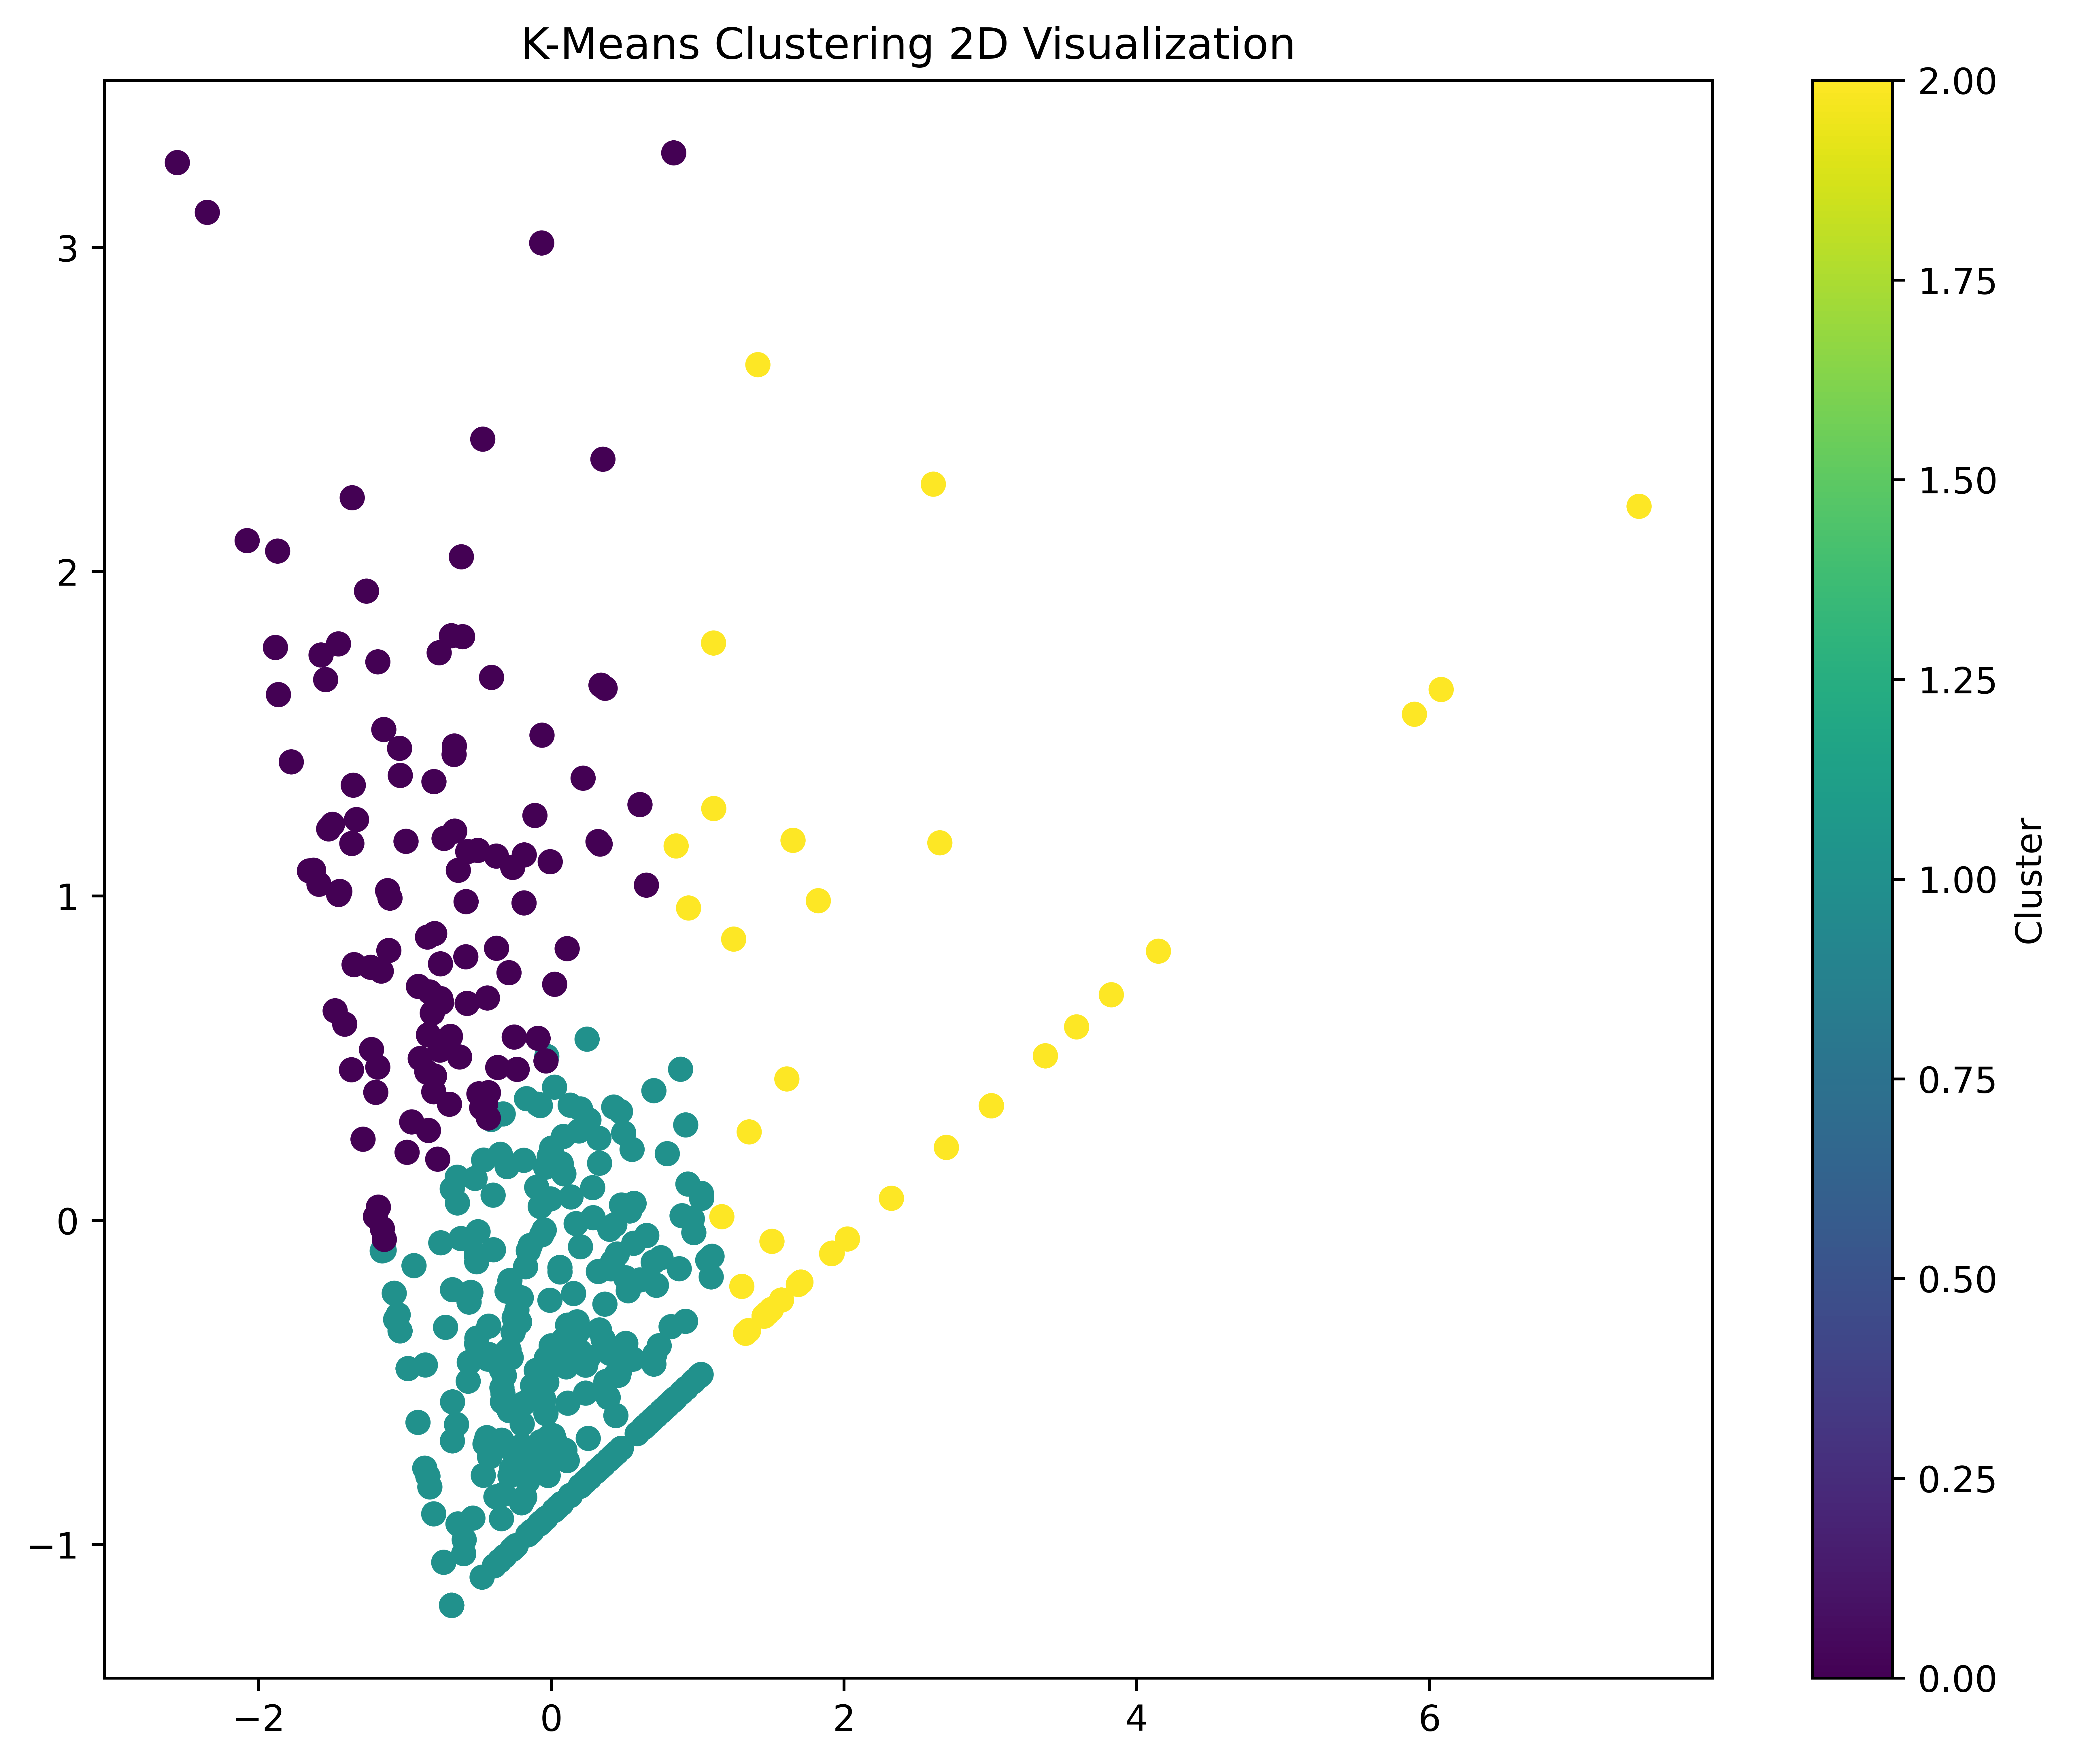
\includegraphics[width=\textwidth]{../data/charts/kmeans_2d.png}
        \caption{2D cluster visualization}
        \label{fig:kmeans_2d}
    \end{subfigure}
    \hfill
    \begin{subfigure}[b]{0.48\textwidth}
        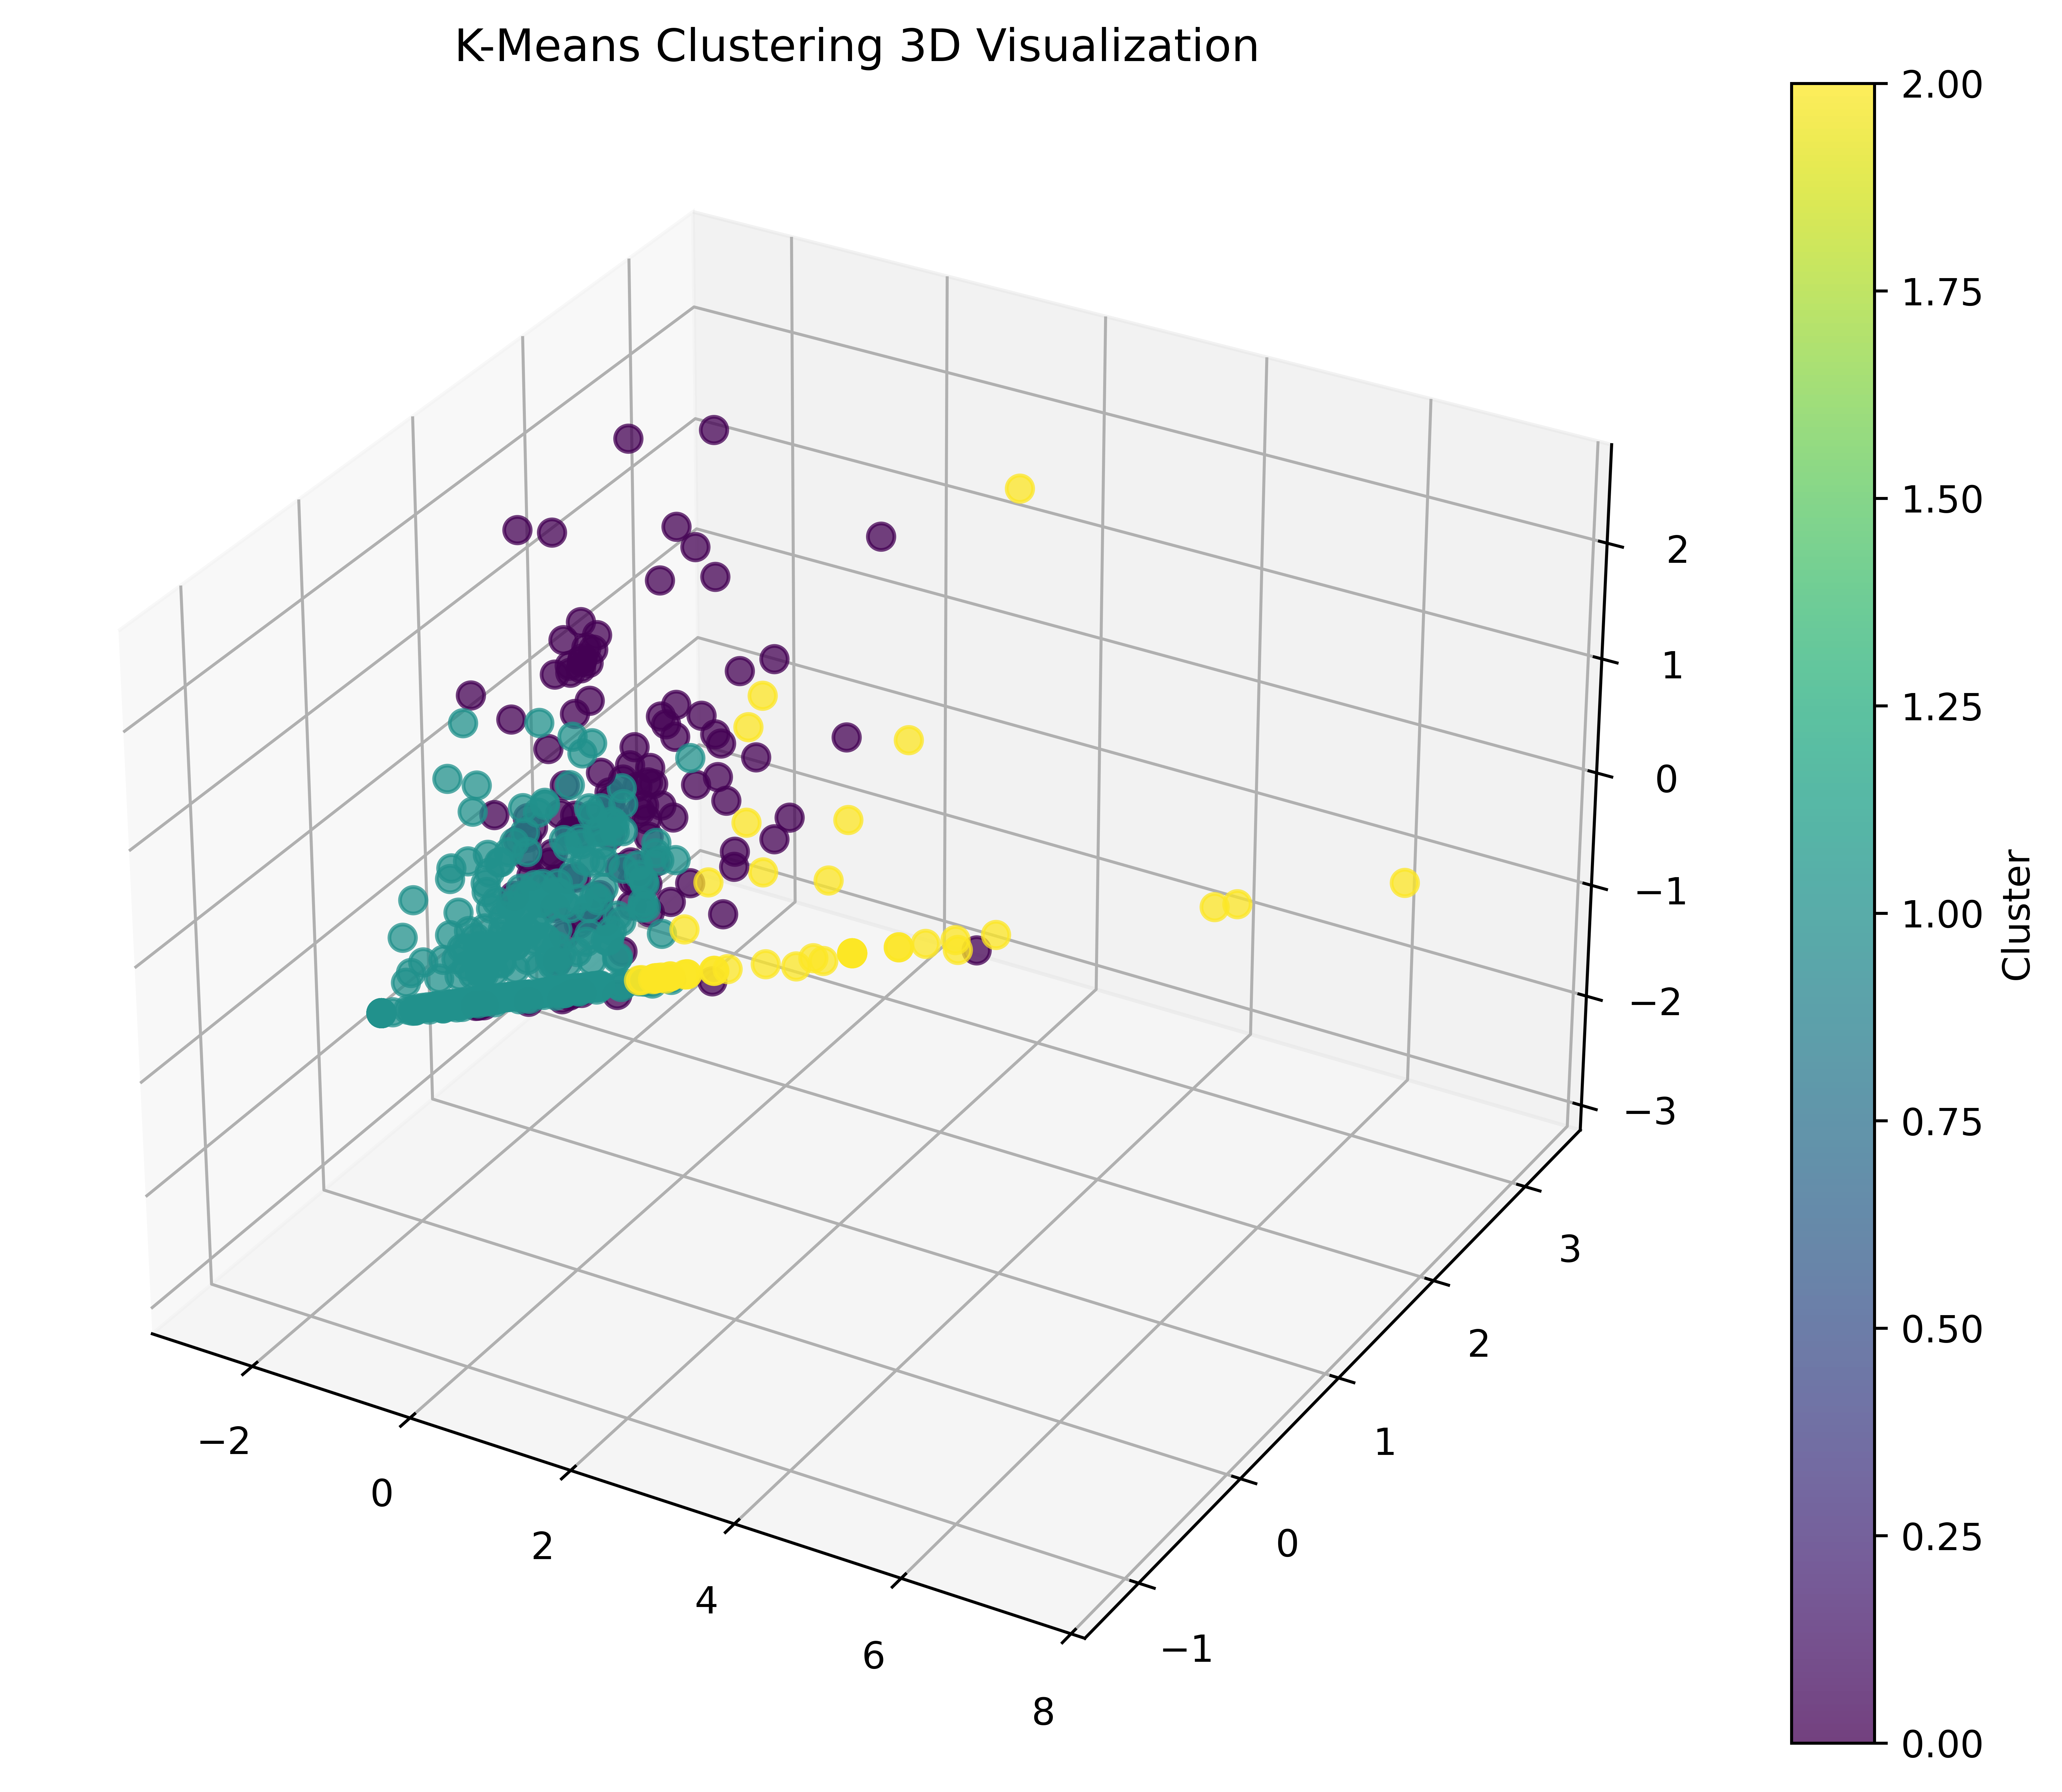
\includegraphics[width=\textwidth]{../data/charts/kmeans_3d.png}
        \caption{3D cluster visualization}
        \label{fig:kmeans_3d}
    \end{subfigure}
    \caption{K-Means clustering results after PCA dimensionality reduction}
    \label{fig:kmeans_viz}
\end{figure}

PCA works by finding principal components---linear combinations of original features that explain the largest variance in the data. The first two principal components typically capture the majority of information, enabling approximate cluster structure representation on a plane.


\section{Player Valuation with XGBoost}

\subsection{Objective}

Build a regression model to predict player transfer values based on match statistics, using XGBoost combined with Optuna hyperparameter optimization.

\subsection{Methodology}

\subsubsection{Data Loading and Merging --- \texttt{core/loader.py}}

Data from the \texttt{statistic} and \texttt{price} tables in SQLite is combined via a \texttt{LEFT JOIN} on the \texttt{Player} field. Squad-level descriptive statistics (\texttt{squad\_stats\_summary.csv}) are then merged on the \texttt{Squad} field, providing team-level context for each player.

\subsubsection{Feature Engineering --- \texttt{core/features.py}}

The feature design process encompasses multiple groups:

\begin{enumerate}
    \item \textbf{Target Variable Processing:} Transfer values are extracted from strings (removing \texteuro{} and M symbols), converted to numeric type. Players without price data are dropped.
    
    \item \textbf{Position Encoding:} The \texttt{Pos} column (which may contain multiple comma-separated positions) is One-Hot encoded, creating binary variables for each position.
    
    \item \textbf{Player-Level Features:}
    \begin{itemize}
        \item $\texttt{Squad\_Status} = \texttt{Starts} / \texttt{MP}$ --- starting ratio.
        \item $\texttt{Stamina\_Trust} = \texttt{Min} / \texttt{MP}$ --- average minutes per match.
        \item $\texttt{NPG\_Efficiency} = (\texttt{Gls} - \texttt{PK}) / \texttt{Min}$ --- non-penalty goal efficiency.
        \item $\texttt{Discipline\_Risk} = (\texttt{CrdY} + 2 \times \texttt{CrdR}) / \texttt{Min}$ --- discipline risk.
        \item $\texttt{Assist\_Efficiency} = \texttt{Ast} / \texttt{Min}$ --- assist efficiency.
    \end{itemize}
    
    \item \textbf{Squad-Level Features:}
    \begin{itemize}
        \item $\texttt{Min\_Z\_Score}$ --- Z-score of playing time relative to squad.
        \item $\texttt{Age\_Diff\_Squad}$ --- age difference from squad average.
        \item $\texttt{Offensive\_Share\_Proxy}$ --- individual offensive contribution ratio.
        \item $\texttt{Squad\_Age\_Profile}$, $\texttt{Squad\_Rotation\_Index}$, $\texttt{Squad\_Discipline}$ --- tactical characteristics of the squad.
    \end{itemize}
\end{enumerate}

\subsubsection{Model Training --- \texttt{core/training.py}}

\textbf{Log Transformation:} The target variable (transfer value) follows a strongly right-skewed distribution. A $\log(1+x)$ transformation is applied to approximate normality, improving regression model performance.

\textbf{XGBoost Algorithm:} eXtreme Gradient Boosting is an ensemble method based on gradient boosting that sequentially builds decision trees, where each new tree learns from the residuals of the preceding ensemble. Key regularization mechanisms include:

\begin{itemize}
    \item \textbf{Monotone Constraints:} Enforce logical relationships (e.g., more goals $\Rightarrow$ higher value, more cards $\Rightarrow$ lower value).
    \item \textbf{Interaction Constraints:} Limit interactions between feature groups (attacking, fitness, discipline) to prevent overfitting on meaningless combinations.
    \item \textbf{L1/L2 Regularization:} \texttt{reg\_alpha} and \texttt{reg\_lambda} control model complexity.
\end{itemize}

\textbf{Hyperparameter Optimization with Optuna:} The Optuna framework uses the Tree-structured Parzen Estimator (TPE)---a Bayesian optimization method---to intelligently search the hyperparameter space. Cross-validation uses \texttt{RepeatedStratifiedKFold} ($k=5$, 3 repeats) with stratification by value quantiles (\texttt{qcut} with 10 bins), ensuring each fold has a similar transfer value distribution.

\begin{table}[H]
\centering
\caption{Optuna hyperparameter search space}
\label{tab:optuna_space}
\begin{tabular}{l l l}
\toprule
\textbf{Group} & \textbf{Parameter} & \textbf{Range} \\
\midrule
Optimization     & learning\_rate       & $[10^{-3}, 0.5]$ (log) \\
                 & objective            & squarederror / pseudohubererror \\
\midrule
Regularization   & min\_split\_loss     & $[10^{-4}, 10]$ (log) \\
                 & reg\_alpha            & $[10^{-3}, 100]$ (log) \\
                 & reg\_lambda           & $[10^{-8}, 100]$ (log) \\
\midrule
Tree Structure   & max\_depth            & $[2, 7]$ \\
                 & min\_child\_weight    & $[1, 15]$ \\
\midrule
Sampling         & subsample            & $[0.1, 1.0]$ (log) \\
                 & colsample\_bytree    & $[0.1, 1.0]$ (log) \\
\bottomrule
\end{tabular}
\end{table}

\subsubsection{Model Evaluation --- \texttt{evaluation.py}}

The model is evaluated on the test set (20\% of data) with three metrics:

\begin{itemize}
    \item \textbf{RMSE} (Root Mean Squared Error): Measures average error, sensitive to large errors.
    \item \textbf{MAE} (Mean Absolute Error): Measures average absolute error.
    \item \textbf{R\textsuperscript{2}} (Coefficient of Determination): Proportion of variance explained by the model.
\end{itemize}

A Dummy Regressor (predicting the mean value) serves as a baseline for comparison, ensuring XGBoost learns genuine relationships in the data rather than just memorizing central tendencies.

\subsection{Results}

Three chart types are automatically generated:

\begin{figure}[H]
    \centering
    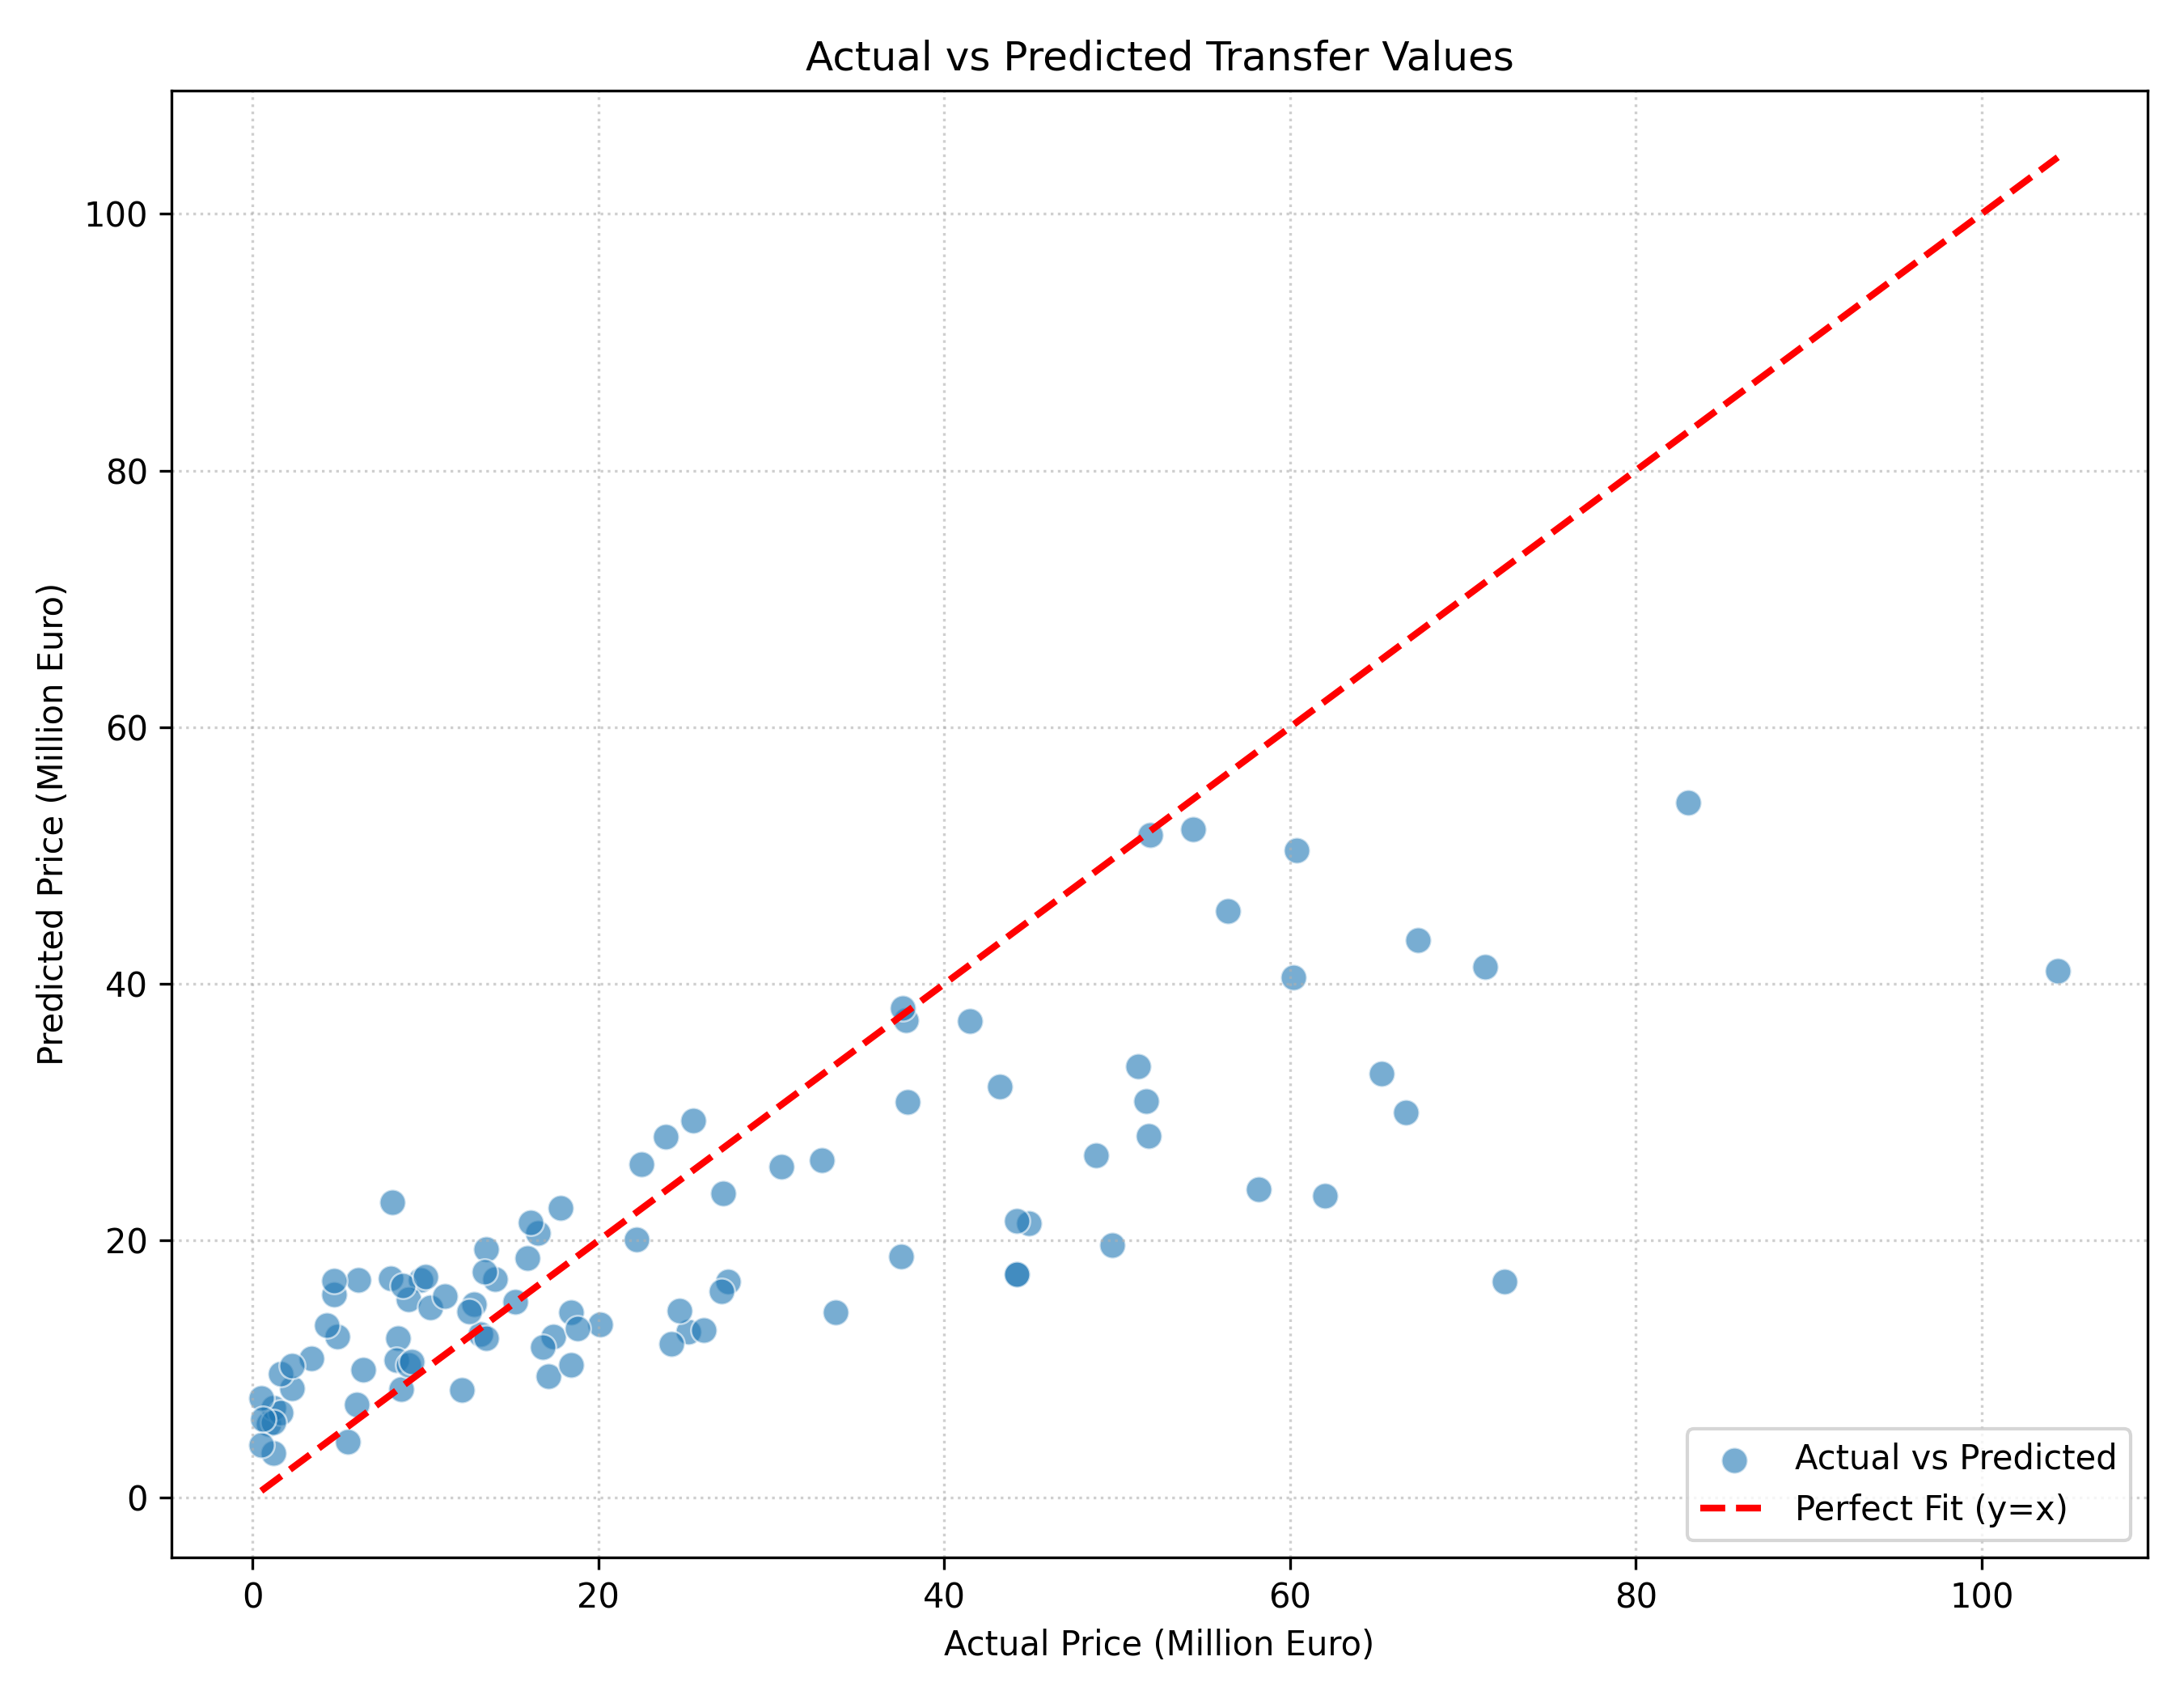
\includegraphics[width=0.7\textwidth]{../data/charts/actual_vs_predicted.png}
    \caption{Actual vs.\ predicted transfer values. The dashed red line represents perfect fit ($y = x$).}
    \label{fig:actual_vs_predicted}
\end{figure}

\begin{figure}[H]
    \centering
    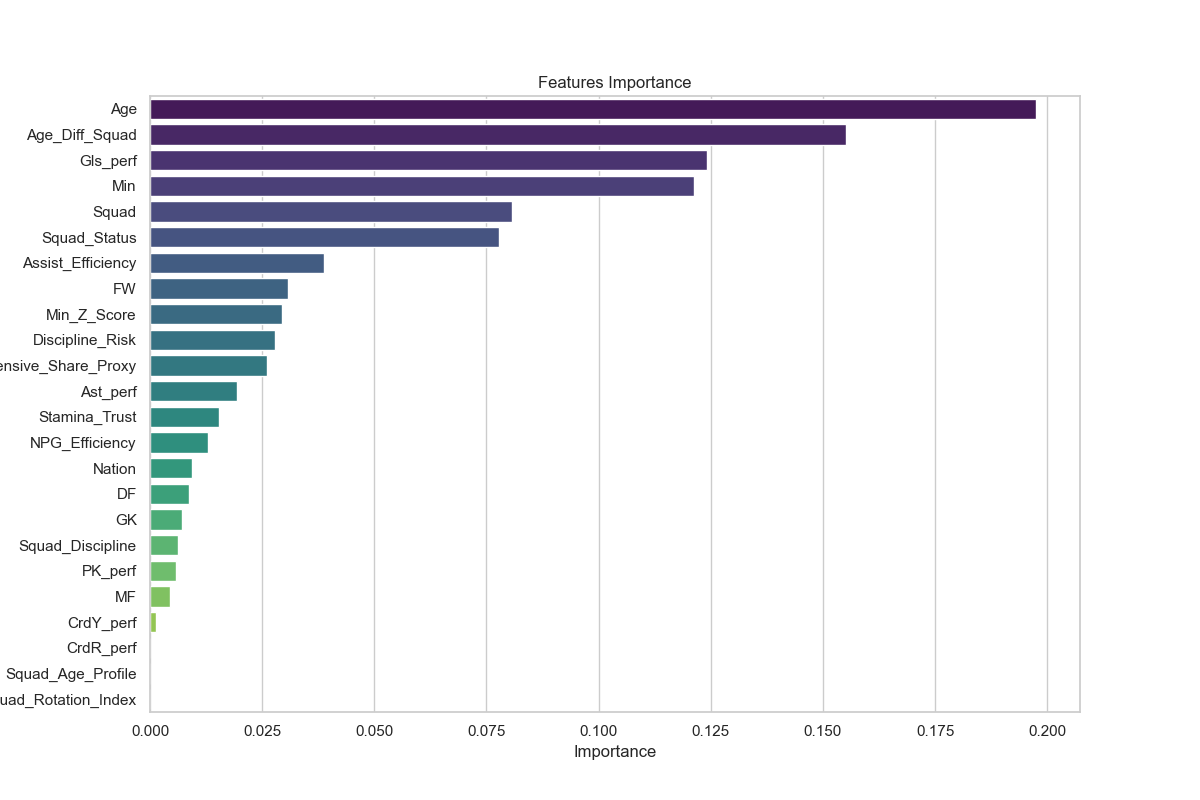
\includegraphics[width=0.75\textwidth]{../data/charts/feature_importance.png}
    \caption{Feature importance in the final XGBoost model}
    \label{fig:feature_importance}
\end{figure}

\begin{figure}[H]
    \centering
    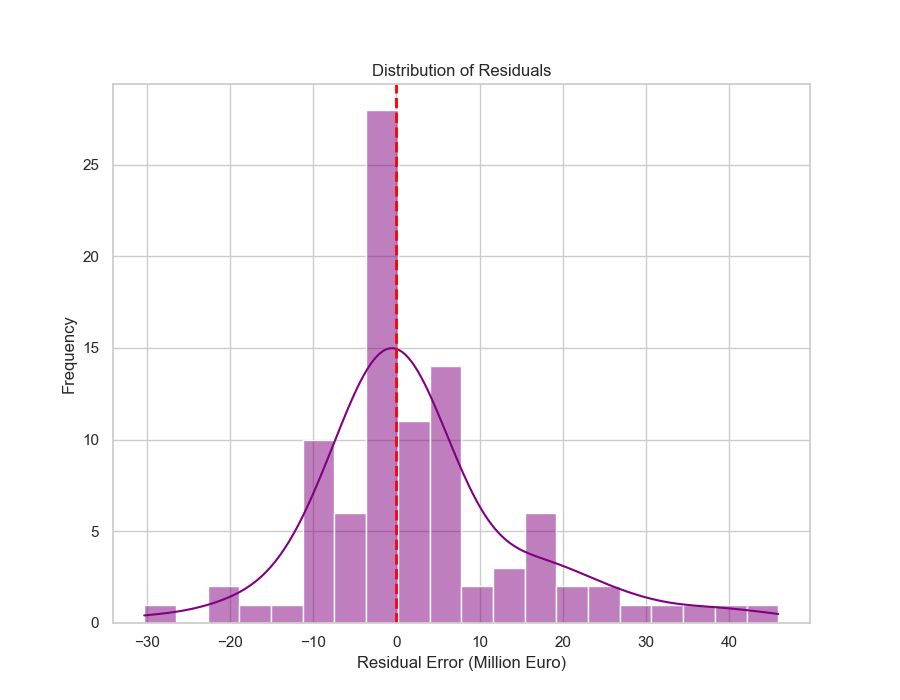
\includegraphics[width=0.7\textwidth]{../data/charts/residual_analysis.png}
    \caption{Residual distribution. A near-symmetric distribution around zero indicates no systematic bias.}
    \label{fig:residuals}
\end{figure}

Each test-set player is classified as \textit{Undervalued}, \textit{Overvalued}, or \textit{Fair Valued}. Detailed results are exported to \texttt{player\_valuation\_results.xlsx}.


% =============================================================
% CHAPTER 6: CONCLUSION
% =============================================================
\chapter{Conclusion}

\section{Summary}

This project successfully completed all three required phases:

\begin{enumerate}
    \item \textbf{Data Crawling:} The automated crawling system using SeleniumBase (UC mode) successfully collected match statistics and transfer valuations from two online sources, handling technical challenges including anti-bot mechanisms, dynamic content loading, and fuzzy name matching.
    
    \item \textbf{Lookup Application:} The Flask RESTful API and CLI client provide a flexible lookup interface, supporting partial-match search and multi-format output (JSON, terminal tables, CSV).
    
    \item \textbf{Analytics and Machine Learning:} Squad-level descriptive statistics combined with a weighted ranking model enable comprehensive performance assessment. K-Means clustering (with $k$ selected via Elbow and Silhouette methods) successfully groups players by playing style. The XGBoost model with Optuna optimization predicts transfer values based on performance data.
\end{enumerate}

\section{Limitations}

\begin{itemize}
    \item Dataset size is limited to a single season, affecting model generalizability.
    \item Transfer values are influenced by many off-pitch factors (brand, contract length, age) that match statistics do not fully capture.
    \item The clustering model uses four features; this could be expanded to capture more playing-style dimensions.
\end{itemize}

\section{Future Work}

\begin{itemize}
    \item Expand data collection across multiple seasons and leagues to increase sample size.
    \item Integrate advanced metrics (expected goals, progressive passes) from supplementary sources.
    \item Develop an interactive web dashboard for the lookup and visualization modules.
    \item Experiment with alternative model architectures (LightGBM, CatBoost, Neural Networks) for performance comparison.
\end{itemize}


% =============================================================
% REFERENCES
% =============================================================
\begin{thebibliography}{9}

\bibitem{fbref}
Sports Reference LLC, ``FBref.com --- Football Statistics and History,''
\url{https://fbref.com/en/}, accessed April 2026.

\bibitem{fbtransfers}
Football Transfers, ``Player Valuations and Transfer Data,''
\url{https://www.footballtransfers.com}, accessed April 2026.

\bibitem{xgboost}
T. Chen and C. Guestrin, ``XGBoost: A Scalable Tree Boosting System,''
in \textit{Proc. 22nd ACM SIGKDD Int. Conf. Knowledge Discovery and Data Mining}, 2016, pp. 785--794.

\bibitem{optuna}
T. Akiba, S. Sano, T. Yanase, T. Ohta, and M. Koyama,
``Optuna: A Next-generation Hyperparameter Optimization Framework,''
in \textit{Proc. 25th ACM SIGKDD Int. Conf. Knowledge Discovery and Data Mining}, 2019, pp. 2623--2631.

\bibitem{kmeans}
J. MacQueen, ``Some Methods for Classification and Analysis of Multivariate Observations,''
in \textit{Proc. Fifth Berkeley Symp. Mathematical Statistics and Probability}, vol. 1, 1967, pp. 281--297.

\bibitem{sklearn}
F. Pedregosa \textit{et al.}, ``Scikit-learn: Machine Learning in Python,''
\textit{J. Machine Learning Research}, vol. 12, pp. 2825--2830, 2011.

\bibitem{selenium}
SeleniumBase, ``SeleniumBase --- Browser Automation Framework,''
\url{https://github.com/seleniumbase/SeleniumBase}, accessed April 2026.

\end{thebibliography}

\end{document}

